\question 下图示意了发送者利用非对称加密算法向接收者传送消息的过程,图中a和b处分别是(
~)。

~
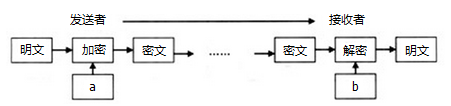
\includegraphics[width=3.33333in,height=0.78125in]{computerassets/BC3B8D19EE7AB6B46BF4430685BA419B.png}
\par\fourch{\textcolor{red}{发送者的私钥,发送者的公钥}}{发送者的公钥,接收者的私钥}{发送者的私钥,接收者的公钥}{接收者的私钥,接收者的公钥}
\begin{solution}在公钥加密系统中,如果要实现所发送的消息供公众阅读,则需发送者使用自身的私钥对所传送的消息进行加密,接收者从安全证书中心获取的发送者的公钥对密文进行解密。另外,在公钥加密系统中,发送者还可以使用从安全证书中心获取的接收者的公钥对所传送的消息进行加密,接收者使用其本身的私钥对该密文进行解密。从而实现所发送的消息只提供给指定接收者阅读的功能。由于本题四个选项中未出现``接收者的公钥,接收者的私钥'',因此只有选项A是正确答案。
\end{solution}
